\documentclass[a4paper,12pt]{article}
\usepackage[utf8]{inputenc}
\usepackage[T1]{fontenc}
\usepackage[french]{babel}
\usepackage{graphicx}
\usepackage{listings}
\usepackage{xcolor}
\usepackage{hyperref}
\usepackage{fullpage}
\usepackage{placeins}
\graphicspath{{images/}}

\lstset{
    basicstyle=\ttfamily\small,
    frame=single,
    breaklines=true,
    postbreak=\mbox{\textcolor{red}{$\hookrightarrow$}\space},
    columns=fullflexible,
    showstringspaces=false
}

\begin{document}


\section{Introduction}
Ce projet implémente un système de chat distribué en Java, utilisant RMI (Remote Method Invocation) et l'algorithme d'horodatage logique de Lamport. L'objectif est de permettre à plusieurs clients de communiquer en temps réel tout en garantissant la cohérence et l'ordre causal des messages, même dans un environnement distribué.

\section{Présentation du Projet}
Le système se compose de plusieurs clients (interface graphique ou ligne de commande) et d'un serveur centralisé, pouvant être déployé dans un conteneur Docker. Les clients se connectent au serveur, envoient et reçoivent des messages, et chaque événement (envoi/réception) est horodaté grâce à l'algorithme de Lamport.

\begin{figure}[ht!]
    \centering
    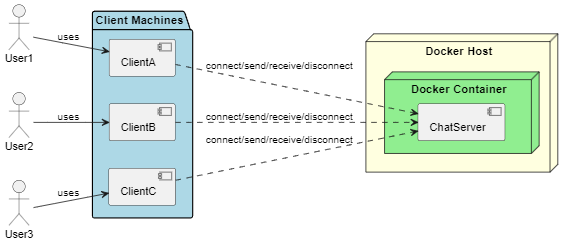
\includegraphics[width=1\textwidth]{architecture.png}
    \caption{Architecture générale du système distribué}
\end{figure}

\textbf{L'architecture comprend:}
\begin{itemize}
    \item Des clients (A, B, C) utilisés par différents utilisateurs;
    \item Un serveur de chat centralisé, déployé dans un conteneur Docker;
    \item Des échanges de messages via RMI, avec gestion des connexions, envois, réceptions et déconnexions.
\end{itemize}

\textbf{Contraintes d'implémentation:}
\begin{itemize}
    \item L'historique des messages sur le serveur est limité à 50 messages pour garantir de bonnes performances~; lorsqu'un nouveau message arrive alors que la limite est atteinte, le plus ancien des 50 messages est supprimé pour faire de la place au nouveau;
    \item Deux utilisateurs ne peuvent pas se connecter avec le même nom~: le serveur impose l'unicité des noms d'utilisateur.
\end{itemize}

\section{Diagramme de Classes}
Le diagramme suivant présente les principales classes et interfaces du projet, incluant la gestion des clients, du serveur, des messages et de l'horloge de Lamport.

\begin{figure}[ht!]
    \centering
    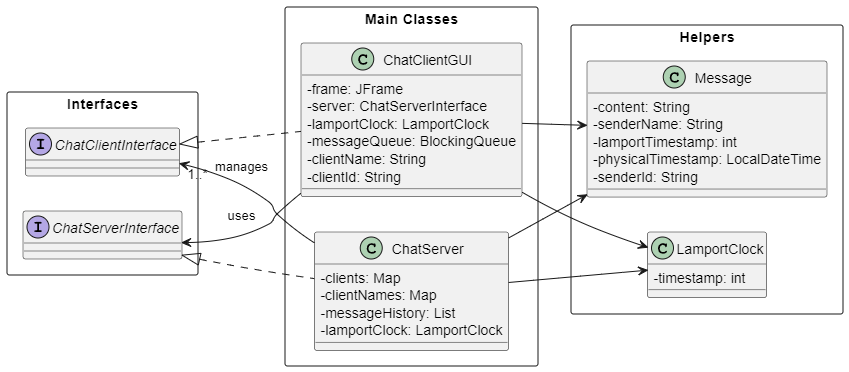
\includegraphics[width=1\textwidth]{class.png}
    \caption{Diagramme de classes du système de chat distribué}
\end{figure}
\FloatBarrier\


\section{Algorithme de Lamport: Présentation et Fonctionnement}
L'algorithme de Lamport permet d'ordonner les événements dans un système distribué à l'aide d'horodatages logiques. Chaque processus (client ou serveur) possède une horloge Lamport (un entier). Les règles sont:
\begin{enumerate}
    \item Avant chaque événement local (envoi de message), le processus incrémente son horloge;
    \item Lorsqu'un message est envoyé, il est accompagné de la valeur courante de l'horloge;
    \item À la réception d'un message, le processus met à jour son horloge à \\\texttt{max (son\_horloge, horloge\_reçue) + 1}.
\end{enumerate}

\subsection{Présentation de l'algorithme}
L'algorithme de Lamport, proposé par Leslie Lamport en 1978, vise à résoudre le problème de l'ordre des événements dans un système distribué où il n'existe pas d'horloge physique globale. Dans un tel environnement, il est difficile de déterminer l'ordre exact des événements (comme l'envoi ou la réception de messages) car chaque machine possède sa propre horloge locale. L'algorithme introduit le concept d'horodatage logique: chaque événement se voit attribuer un numéro croissant, garantissant ainsi un ordre partiel cohérent entre tous les nœuds du système. Cela permet d'assurer la cohérence causale des messages et d'éviter les conflits liés à la simultanéité des actions dans le système distribué.
\begin{lstlisting}
class LamportClock {
    int compteur = 0;

    // Incrementer pour chaque evenement local (envoi de message)
    synchronized int tick() {
        return ++compteur;
    }

    // Mettre a jour lors de la reception d'un message
    synchronized void update(int horlogeRecue) {
        compteur = max(compteur, horlogeRecue) + 1;
    }

    // Obtenir la valeur courante
    synchronized int get() {
        return compteur;
    }
}
\end{lstlisting}

\subsection{Étapes de l'algorithme dans le chat}
\begin{enumerate}
    \item Le client A veut envoyer un message: il incrémente son horloge, puis envoie le message avec l'horodatage;
    \item Le serveur reçoit le message, met à jour sa propre horloge, puis diffuse le message aux autres clients;
    \item Le client B reçoit le message, met à jour son horloge selon la règle de Lamport;
    \item À chaque nouvel événement (envoi/réception), l'horloge est ajustée pour garantir l'ordre causal.
\end{enumerate}

\begin{figure}[ht!]
    \centering
    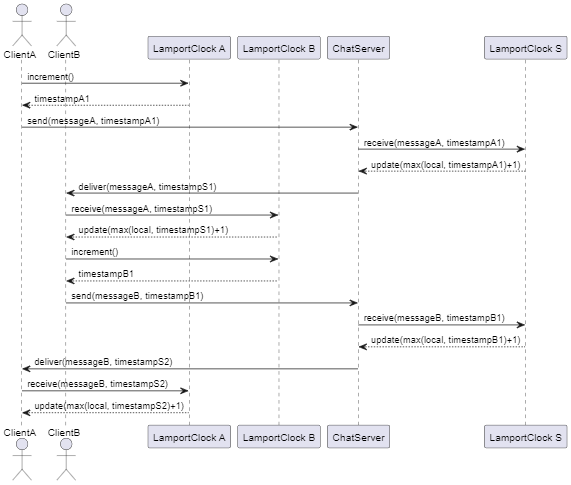
\includegraphics[width=1\textwidth]{sequence.png}
    \caption{Diagramme de séquence illustrant l'algorithme de Lamport dans le chat}
\end{figure}
\FloatBarrier\

\section{Interface Utilisateur}
Cette section présente les différentes interfaces du système de chat distribué, montrant l'évolution de l'interface graphique selon les actions des utilisateurs.

\subsection{Interface de connexion}
Lorsqu'un utilisateur lance le client, il doit d'abord saisir son nom d'utilisateur pour se connecter au serveur.

\begin{figure}[ht!]
    \centering
    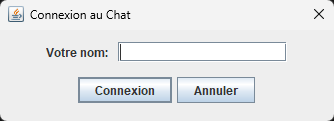
\includegraphics[width=0.8\textwidth]{name.png}
    \caption{Interface de saisie du nom d'utilisateur}
\end{figure}
\FloatBarrier\

\subsection{Interface principale vide}
Après la connexion, l'utilisateur accède à l'interface principale du chat, initialement vide.

\begin{figure}[ht!]
    \centering
    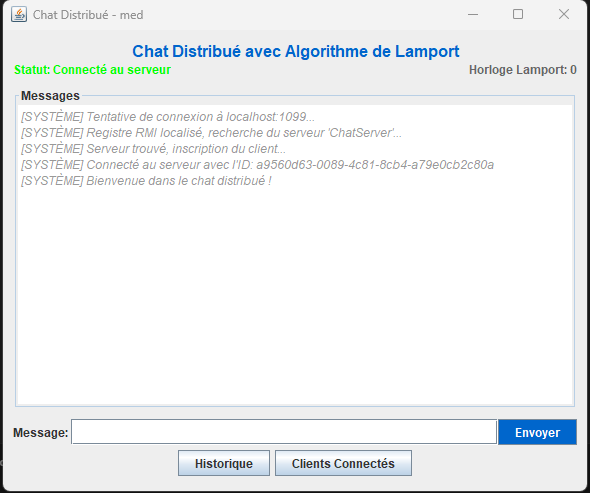
\includegraphics[width=0.8\textwidth]{chatEmpty.png}
    \caption{Interface principale du chat après connexion (vide)}
\end{figure}
\FloatBarrier\
\subsection{Liste des clients connectés}
L'interface affiche la liste des utilisateurs actuellement connectés au serveur de chat.

\begin{figure}[ht!]
    \centering
    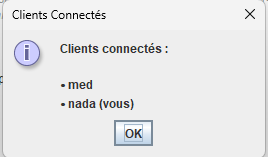
\includegraphics[width=0.8\textwidth]{connectedClients.png}
    \caption{Affichage de la liste des clients connectés}
\end{figure}
\FloatBarrier\
\subsection{Historique des messages}
L'interface permet de visualiser l'historique des messages échangés, avec les horodatages de Lamport.
(L'historique est limité aux 50 derniers messages)
\begin{figure}[ht!]
    \centering
    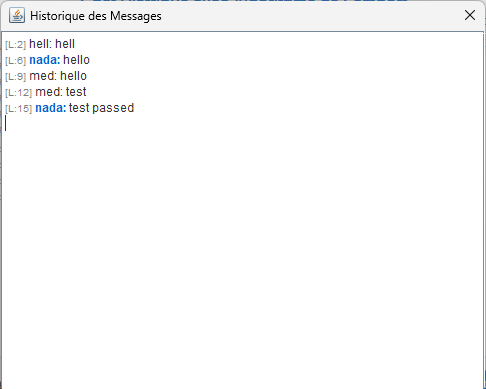
\includegraphics[width=0.8\textwidth]{history.png}
    \caption{Affichage de l'historique des messages avec horodatages}
\end{figure}
\FloatBarrier\
\subsection{Communication entre plusieurs clients}
L'interface montre la communication en temps réel entre plusieurs utilisateurs connectés simultanément.

\begin{figure}[ht!]
    \centering
    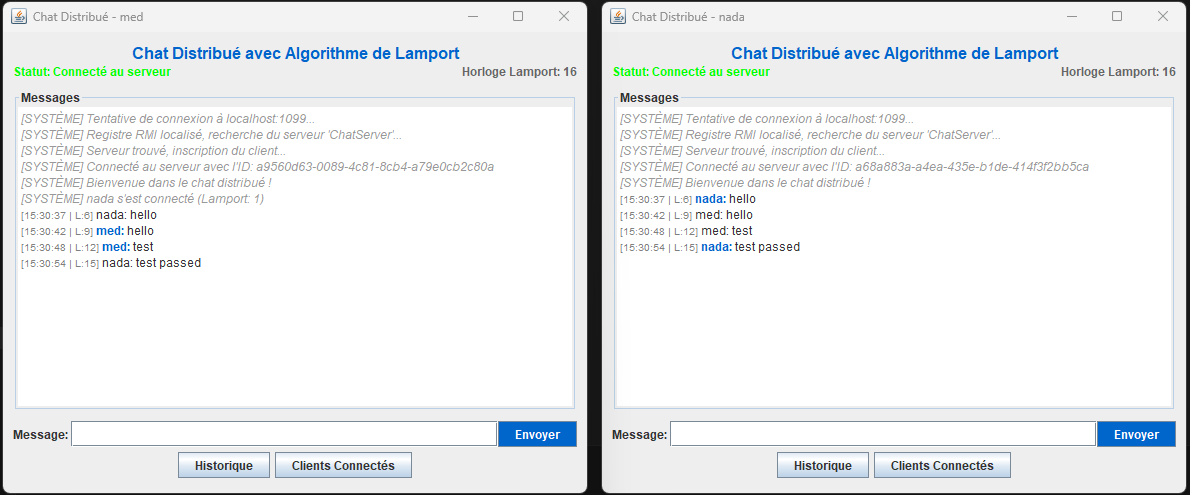
\includegraphics[width=1\textwidth]{twoClients.png}
    \caption{Communication entre plusieurs clients connectés}
\end{figure}
\FloatBarrier\

\section{comment executer le projet}

\subsection{Lancer le serveur avec Docker}
\begin{enumerate}
    \item Assurez-vous d'avoir Docker et Docker Compose installés sur votre machine;
    \item Ouvrez un terminal dans le dossier du projet contenant le fichier \\\texttt{docker-compose.yml};
    \item Lancez le serveur avec la commande suivante:
    \begin{lstlisting}[language=bash]
docker-compose up -d
    \end{lstlisting}
    \item Pour vérifier que le serveur fonctionne, vous pouvez consulter les logs:
    \begin{lstlisting}[language=bash]
docker-compose logs -f
    \end{lstlisting}
    \item Le serveur de chat est maintenant prêt à accepter des connexions clients.
\end{enumerate}

\subsection{Lancer un client GUI (Windows)}
\begin{enumerate}
    \item Ouvrez un terminal PowerShell dans le dossier du projet;
    \item Exécutez le script PS suivant pour démarrer l'interface graphique du client:
    \begin{lstlisting}[language=bash]
./start-client-gui.ps1
    \end{lstlisting}
    \item Suivez les instructions à l'écran pour vous connecter au serveur. L'utilisateur doit uniquement saisir son nom; l'adresse et le port du serveur sont automatiquement récupérés depuis le fichier \texttt{config.properties};
    \item Vous pouvez ouvrir plusieurs terminaux et lancer plusieurs clients pour simuler plusieurs utilisateurs.
\end{enumerate}

\section{Conclusion}
Ce projet démontre l'utilisation de l'algorithme de Lamport pour assurer la cohérence des messages dans un système de chat distribué. Grâce à l'architecture modulaire et à l'intégration de Docker, le système est facilement déployable et extensible.

\end{document}
